\subsection{Curvas e conexidade}

Se na seção anterior, por um lado, compreendemos uma curva de um ponto $p$ até outro $q$ como uma ``deformação'' de $p$ resultando em $q$, então nesta seção, por outro lado, compreenderemos uma curva entre $p$ e $q$ como um ``caminho'' que conecta $p$ e $q$ em um dado espaço. Veremos a seguir como desfrutar desta intuição sobre curvas.

\vspace{0.5em}

\begin{definition}
    Sejam $p$ e $q$ pontos quaisquer em $X$. Um \emph{caminho} de $p$ até $q$ é uma curva de $p$ até $q$ definida em $[0, 1]$, i.e.\@ uma função $\alpha : I \to X$ sujeita às condições:%
    \linebreak\vspace{-1.2em}
%
    \begin{enumerate}
    [
        itemsep=0pt,
        label={(\roman*)}
    ]
        \item
        $\alpha$ é contínua.

        \item
        $\alpha(0) = p$

        \item
        $\alpha(1) = q$
        \qedalt
    \end{enumerate}
\end{definition}

\begin{remark}
    Note que toda curva $[a, b] \to X$ definida em um intervalo fechado $[a, b] \subseteq \R$ arbitrário pode ser dada, de maneira equivalente, por um caminho $I \to X$, e em particular $t \mapsto (1 - t) \cdot a + t \cdot b$ é um homeomorfismo entre $I$ e $[a, b]$.
    \qedalt
\end{remark}

% exemplos, E, B^{n + 1}, S^n

\begin{comment}

Como dito no Comentário 1.1, podemos enxergar homotopias como curvas entre funções contínuas, e como vimos nos exemplos da seção anterior, curvas ocorrem naturalmente nos componentes de uma homotopia e entre as funções contínuas cujas homotopias são estudadas. Como curvas são de importância para a teoria das homotopias, definimos a seguir algumas noções convenientes para falar sobre curvas.%
\linebreak\vspace{-1.2em}

    Existe uma operação muito importante entre curvas, denominada \emph{concatenação}, e que basicamente consiste em ``colar'' duas curvas em uma extremidade em comum. Em maior detalhe, se $\alpha : p \pathto q$ e $\beta : q \pathto r$ são curvas em $X$ compartilhando uma mesma extremidade $q$, então a concatenação de $\alpha$ e $\beta$ é uma curva $\alpha \cdot \beta : p \pathto r$ entre as extremidades restantes, $p$ e $r$, interceptando o ponto $q$, e contendo ambas $\alpha$ e $\beta$.%
\linebreak\vspace{-1.2em}

\begin{figure}[htpb]
\centering
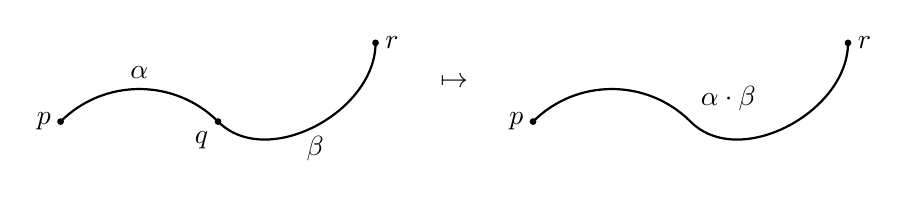
\begin{tikzpicture}
    \draw [thick]
        (-2,-1)
        to[out=45,in=135]
            node [above] {$\alpha$}
        (0,-1)
        ;

    \draw [thick]
        (0,-1)
        to[out=-45,in=-90]
            node [below] {$\beta$}
        (2,0)
        ;

    \draw [fill]
        (-2,-1) circle (1pt)
            node [left] {$p$}
        (0,-1) circle (1pt)
            node [below left] {$q$}
        (2,0) circle (1pt)
            node [right] {$r$}
        ;

    \node at (3,-0.5) {$\mapsto$};

    \draw [thick]
        (4,-1)
        to[out=45,in=135]
        (6,-1)
            node [above right] {$\alpha \cdot \beta$}
        to[out=-45,in=-90]
        (8,0)
        ;

    \draw [fill]
        (4,-1) circle (1pt)
            node [left] {$p$}
        %(6,-1) circle (1pt)
            %node [below left] {$q$}
        (8,0) circle (1pt)
            node [right] {$r$}
        ;
\end{tikzpicture}
\end{figure}

Existem muitas maneiras equivalentes de parametrizar a concatenação de $\alpha$ e $\beta$ obedecendo à descrição cima, mas uma maneira bem simples e direta é a seguinte:

\vspace{0.5em}

\begin{definition}[(Concatenação)]
    Dados os pontos $p$, $q$ e $r$ e as curvas $\alpha : p \pathto q$ e $\beta : q \pathto r$ em um espaço $X$, denotamos por $\alpha \cdot \beta : p \pathto r$ a curva em $X$ dada por%
    \linebreak\vspace{-0.6em}
%
    \begin{equation*}
        (\alpha \cdot \beta)(t) =
        \begin{cases}
            \alpha(2t) & \text{se $0 \leq t \leq 1/2$} \\
            \beta(2t- 1) & \text{se $1/2 \leq t \leq 1$}
        \end{cases}
    \end{equation*}
%
    para todo $t \in I$, e denominada a \emph{concatenação} de $\alpha$ e $\beta$.
    \qedalt
\end{definition}

Outra operação importante é a \emph{inversão} $\gamma^{-1}$ de uma curva $\gamma$, que consiste apenas em reparametrizar $\gamma$ de tal modo que, se $\gamma : p \pathto q$ então $\gamma^{-1} : q \pathto p$; em palavras, de modo que a ``orientação'' de $\gamma$ seja invertida em $\gamma^{-1}$. Obtemos a definição de $\gamma^{-1}$:%
\linebreak\vspace{-1.2em}

\vspace{0.5em}

\begin{definition}[(Curvas inversas)]
    Dada uma curva $\gamma : p \pathto q$ em $X$, definimos por
%
    \begin{equation*}
        \gamma^{-1}(t) = \gamma(1 - t)
    \end{equation*}
%
    para todo $t \in I$ uma curva em $X$, denominada a \emph{curva inversa} de $\gamma$.
    \qedalt
\end{definition}

\begin{remark}
    Caso uma curva $\gamma$ seja uma bijeção, então devemos tomar cuidado para discernir entre a função inversa de $\gamma$ e a curva inversa de $\gamma$; ou seja, entre a inversa de $\gamma$ \emph{como uma função} e a inversa de $\gamma$ \emph{como uma curva}.
    \qedalt
\end{remark}

Por fim, uma curva um tanto trivial mas ocorrendo naturalmente nos exemplos da seção anterior é a \emph{curva constante} em um ponto. Sua definição também é óbvia:%
\linebreak\vspace{-1.2em}

\vspace{0.5em}

\begin{definition}[(Curva constante)]
    Dado um ponto qualquer $p$ em $X$, definimos por
%
    \begin{equation*}
        \msf{const}_p(t) = p
    \end{equation*}
%
    para todo $t \in I$ a \emph{curva constante} em $p$.
    \qedalt
\end{definition}

Obtemos imediatamente o seguinte resultado sobre pontos conectados por curvas:

\vspace{0.5em}

\begin{proposition}
    $\pathto$ é uma relação de equivalência entre pontos; mais precisamente:%
    \linebreak\vspace{-1.2em}
%
    \begin{enumerate}
    [
        itemsep=0pt,
        label={(\roman*)}
    ]
        \item
        $\msf{const}_p : p \pathto p$, pela Definição 1.4.

        \item
        $\gamma : p \pathto q$ $\implies$ $\gamma^{-1} : q \pathto p$, pela Definição 1.3.

        \item
        $\alpha : p \pathto q$, $\beta : q \pathto r$ $\implies$ $\alpha \cdot \beta : p \pathto r$, pela Definição 1.2.
        \qedalt
    \end{enumerate}
\end{proposition}

{\color{red} exemplos: $\R \setminus \{ 0 \}$ e $\R^2 \setminus \{ (0, 0) \}$}

{\color{red} definição: conexidade por curvas}

{\color{red} proposição: conexidade por curvas $\implies$ conexidade}

\begin{convention}
    Dadas $f$ e $g$ funções em $C(X, Y)$, denotamos simbolicamente por $\eta : f \sim g$ o juízo de que $\eta$ é uma homotopia de $f$ até $g$, no sentido da Definição 1.2, ou ainda por $f \sim g$ se $\eta$ estiver implícita ou puder ser inferida pelo contexto.
    \qedalt
\end{convention}
    
\end{comment}